\documentclass[conference]{IEEEtran}
\usepackage{graphicx}
\usepackage{float}

\graphicspath{ {./images} }
\IEEEoverridecommandlockouts
% The preceding line is only needed to identify funding in the first footnote. If that is unneeded, please comment it out.
\usepackage{cite}
\usepackage{amsmath,amssymb,amsfonts}
\usepackage{algorithmic}
\usepackage{graphicx}
\usepackage{textcomp}
\usepackage{xcolor}
\def\BibTeX{{\rm B\kern-.05em{\sc i\kern-.025em b}\kern-.08em
    T\kern-.1667em\lower.7ex\hbox{E}\kern-.125emX}}
\begin{document}

\title{Data Centric Marketplace: When blockchain reigns over the Cloud\\}

\author{\IEEEauthorblockN{MEHDI Ibrahim}
\IEEEauthorblockA{\textit{Ecole Nationale des Sciences Appliquées Oujda (ENSAO)} \\
\textit{Data Science \& Cloud Computing branch}\\
\textit{University Mohamed Premier (UMP)}\\
60000 Oujda, Morocco \\
email address or ORCID}
\and
\IEEEauthorblockN{SBAI Moussaab}
\IEEEauthorblockA{\textit{Ecole Nationale des Sciences Appliquées Oujda (ENSAO)} \\
\textit{Data Science \& Cloud Computing branch}\\
\textit{University Mohamed Premier (UMP)}\\
60000 Oujda, Morocco \\
email address or ORCID}
\and
\IEEEauthorblockN{MAZLIN Mohamed}
\IEEEauthorblockA{\textit{Ecole Nationale des Sciences Appliquées Oujda (ENSAO)} \\
\textit{Data Science \& Cloud Computing branch}\\
\textit{University Mohamed Premier (UMP)}\\
60000 Oujda, Morocco \\
email address or ORCID}
\and
\IEEEauthorblockN{Prof. Dr.AZGHIOU Kamal}
\IEEEauthorblockA{\textit{Ecole Nationale des Sciences Appliquées Oujda (ENSAO)} \\
\textit{Data Science \& Cloud Computing branch}\\
\textit{University Mohamed Premier (UMP)}\\
60000 Oujda, Morocco \\
email address or ORCID}
}

\maketitle

\begin{abstract}
Data has become increasingly important in today's environment. Data security, processing, and analytics are the foundations of whole enterprises. Along with this revolution, governments have passed laws to control how data is held and used, such as the GDPR on user data protection and privacy, which was enacted by the European Union's parliament and council. This is because consumers have become a company's most precious asset because their consent is necessary to handle any data in order to make educated decisions, solve problems, maintain track of records, and many other features.In this article, we offer a solution that uses a permissioned blockchain-based marketplace to empower anybody with data to participate at the heart of the company in decentralized autonomous organizations. Others can join this group and contribute value to the data without jeopardizing privacy which is achieved by Secure Multi-party computation. On top of that, we provide a method for creating and monitoring the infrastructure where the data is being processed with the help of blockchain built-in smart contracts.
\end{abstract}

\begin{IEEEkeywords}
Data-Marketplace, Cloud, Blockchain, Hyperledger Fabric, IoT.
\end{IEEEkeywords}


\section{Introduction}
Technology in the twenty-first century will be remembered for its data-driven 'gold rush.' Every second of the day, it is generated, but only a small portion of it is appropriately utilized. Companies are clamoring for more data as the regulatory environment tightens and new rules are enacted\cite{voigt2017eu}. This is where a data marketplace may be quite beneficial, and that is exactly what we shall discuss in this article.\\
Selling data is fine, but investing in it is more appealing since it offers the owner more control over what happens to his data as it passes via service providers and other parties who can add value to it with their solutions. Even more intriguing than investing with it is not exposing it to the rest of the peers while yet being able to perform calculations on it. And, because blockchain \cite{di2017blockchain} solutions enable secure immutable ledgers, they are the greatest choice for tracking it at every stage.\\
When it comes to blockchains, there are two issues to consider: scalability and privacy. Permissioned blockchains, such as Hyperledger Fabric \cite{androulaki2018hyperledger}, comes in helpful in this situation. Creating "Channels" subnets will allow our application to expand correctly while also limiting the number of authorized users who may read transaction logs: A channel's blocks are only visible to its registered users.
\section{Background}
In this section, we are presenting an overview about various technologies that are the building blocks for our system.
\subsection{Hyperledger Fabric}

\subsubsection{Overview}
Hyperledger Fabric V1.0 was released by the Linux Foundation in 2017. It is an open-source permissioned blockchain framework. It came to life to provide a secure, scalable and flexible groundwork for industrial blockchain solutions. Fabric got rid of the mining process and made sure that the data in the ledger is only accessed by authorized members by creating subnets in the network called Channels. Peers can join a channel (or multiple channels at the same time) by enrolling through MSP (Membership Service Provider) and therefore it will have its ledger and chaincodes (smart contracts) installed.
Consensus is achieved in Hyperledger Fabric after three phases: Endorsement, Ordering and Validation.
 \begin{itemize}
     \item \textbf{Endorsement phase:} Endorsing peers will simulate and execute transactions in an isolated environment and then either sign it as endorsed or not. The result is sent back to the transaction initiator.
     \item \textbf{Ordering phase:} Ordering service (also called ordering service nodes) will receive the transaction and the endorsement signatures and determine the order of transactions.
     \item \textbf{Validation phase:} Validating the authenticity and correctness of blocks of transactions
   \end{itemize}

\subsubsection{Events in Hyperledger Fabric}
There are three sorts of events that can be subscribed to in Hyperledger Fabric:
 \begin{itemize}
     \item \textbf{Block events:} Events that are set automatically when a block is committed.
     \item \textbf{Transaction events:} Also set automatically when a transaction is committed.
     \item \textbf{Contract events:} Events explicitly added to the chaincode and is set when the contract is invoked.
   \end{itemize}
By listening for these events, the application can respond without having to initiate a transaction.
In our system, we will use the contract events by setting up an event listener and handler that will
allow us to utilize data included in these notifications to automatically command and control an infrastructure.

\subsection{Secure Multi-party computation}\label{SMPC}
The idea of outsourcing data processing and computing without handing over the keys to it is the basis of our system. We know that fully homomorphic encryption \cite{lee2022privacy}, \cite{gentry2009fully}, allows such privacy, but we also know that it is fully unpractical. It basically goes like this:\\
Alice encrypts her data $Alice_{Data}$and sends it $E_{Alice}(Alice_{Data})$ to Bob, does his computation $f(E_{Alice}(Alice_{Data}))$ and returns the encrypted result $R$. Alice then decrypts $D_{Alice}(R)$ to find out the results.\\
Multi-party computation \cite{goldreich1998secure} on the other hand is a scheme first developed in 1980’s that aims to provide techniques allowing entities to collaboratively calculate a function while keeping their inputs private.\\
Many protocols are being developed to optimise further the performance of such systems. SPDZ \cite{damgaard2013practical}, a universal multiparty computing protocol that is safe against up to n-1 of the n players being corrupted by an active attacker, is an interesting one that can be implemented to ensure data privacy.

\subsection{Distributed autonomous organisations DAOs}
A decentralized autonomous organization \cite{sims2019blockchain} (DAO) is a collection of entities that work together using smart contracts. This implies that all corporate processes, definitions, and restrictions are encoded in the blockchain and cannot be changed.
This type of organisation was inspired by the decentralized cryptocurrencies by not having any central authority controlling all the flow and risking both single points of failure and privacy.As a result, investors may now purchase DAO shares and get tokens that reflect their ownership in the organization and let them to vote on future initiatives.DAOs are established in our system when two parties agree to collaborate. It's worth noting that one or both of them might already be a DAO.

\section{Literature Review}
Numerous blockchain based data marketplaces have been introduced in the last few years, each with its own vision and architecture. In \cite{DBLP:journals/corr/abs-1812-09966},\cite{ozyilmaz2018idmob},\cite{yoo2020blockchain},\cite{DBLP:journals/corr/abs-1811-11462} a decentralized buy/sell architecture based on blockchain have been proposed as the new solution to traditional data markets. It enforces the fair play between the parties by a punishment system for dishonest behaviours. Elimination of central trusted authorities so that owners of data can have control over it. The implementations of immutable ledgers and smart contracts enabled the users to browse and pick with who they want to work. And to ensure data privacy during the transaction so that no one but the authorized parties can see it, various approaches are presented; Proxied URL to JSON files, selling the decryption key to an encrypted database, or by using swarms in Ethereum network as a decentralized storage for example.

In  \cite{inproceedings}, \cite{suliman2019monetization},\cite{7765669} systems are designed for IoT devices by providing a decentralized platform to sell data streams. These infrastructures are characterized by their low-resources, computational power and lack of security and privacy which requires some sort of middle-system that helps compensate for these weaknesses so they can serve multiple buyers at once.
(datapace) took a step forward with what was already done. A mix of different technologies as hyperledger fabric as an immutable ledger, cosmos for token interoperability and Mainflux as an IoT gateway. The trade is done by exchanging tokens for a Proxied URL with an expiration date determined in the transaction.

We can see in these  examples how they all provided a sales marketplace, and at some point the data will be at the other side in plain text with no proof of where it is and how it is being used.
Our approach is different. Firstly, we are not interested in selling data as it has already been done before many times. We took the famous sentence ‘ Data is the new Oil’ to the letter. Any person having an oil field can either sell it and be satisfied with the one time payment, which is not what people do, or can be part of the business and invest with his land. As for data, it is important to ensure privacy and anonymity in the exploitation phase. Secondly, we want a decentralized control and monitoring over the infrastructure where all the business is running through blockchain.


\section{Data ownership centric architecture}

\begin{figure*}[!htb]
  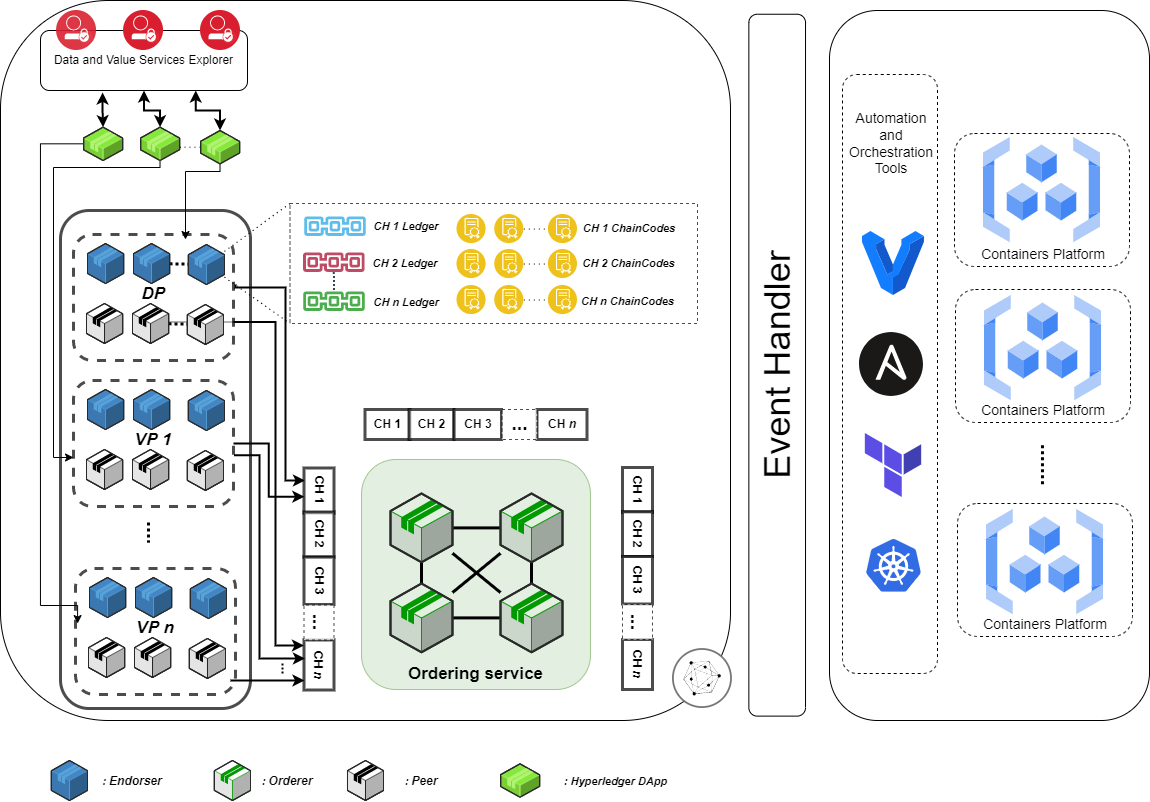
\includegraphics[width=\textwidth]{arch.png}
  \caption{Data ownership centric architecture}
  \label{arch}
\end{figure*}


\subsection{An overview of the proposed architecture}
Here we present a bird’s-eye view of the application and its components. (see figure \ref{arch}
The architecture is mainly composed of two major parts: a Hyperledger Fabric module and an Infrastructure. The communication between the two is made sure by an event handler converting Hyperledger events into commands that will be discussed in section \ref{EvRef}. Our goal is to make any data driven project also data centric, meaning that the data owner can see where his data is being used, how it is being used and also make a profit at the end.

\subsection{The hyperledger part}
The data and value services explorer is where every service will be posted with a detailed description. It is where registration and enrollment will take part since we are in the shadow of a permissioned blockchain (In fabric, when we talk about a blockchain we are referring to a channel). A service is posted by organizations that are composed of either only one peer or more. All the transactions and modifications should go through the ordering service that establishes the total order of all transactions. Multiple channels can be connected to the same ordering service.
In every channel, there is a set of chaincodes that determine the rules of transactions within it, and they will be sending multiple event notifications that go straight to the event listener and handler to command the infrastructure side.

There will be two types of accounts: Data Service Providers and Value Providers. A data service provider is the owner of the data, the value provider is any party that can increase the worth of the data by providing any set of services. The more services are on top of the data layer the more valuable the whole job is.
The channels play a crucial role in keeping privacy inside organizations. For example a data service provider $DSP$ and a value provider $VP_1$ have agreed to work together. Each will invest with his service and will be together in a channel $CH_1=\{DSP, VP_1\}$ that will regulate the workflow using chaincode: Profit splitting, endorsement policies, contract time and other parameters about the workspace and infrastructure. Any other party $VP_2$ wanting to join the ongoing work will join the new channel $CH_2$ with the $CH_1$ still running. The channels’ participants are now : $CH1 =\{DSP, VP_1\}$, $CH_2 =\{DSP, VP_1, VP_2\}$. Each time a new value provider is added, this process will be repeated. For example when $VP_n$ joins, the channels state will be:
\begin{center}
$CH_1$ = $\{DSP, VP_1\}$,\\[5pt]
$CH_2 = \{DSP, VP_1, VP_2\}$,\\[5pt]
$CH_3 = \{DSP, VP_1, VP_2, VP_3\}$,\\[5pt]
	$\vdots$\\[5pt]
$CH_n = \{DSP, VP_1, VP_2, VP_3, … VP_n\}$.
\end{center}

Any party in a channel will have its ledger and chaincodes installed as well as of the later channels. For example the $VP_2$ will have the ledger and chaincodes of $CH_2$ up to $CH_n$. But not $CH_1$ since he is not a member. With that said we see how the data service provider will be the core of the whole project since he takes part in all channels.


\subsection{The infrastructure part}\label{EvRef}
Our two main objectives in this project is to make data the core of the marketplace projects, and to make the blockchain control the workplace where the work is done.Using the HyperledgerFabric chaincode emitted events, we can set up an event listener that will convert json file made by the users containing all the infrastructure details in order to be automatically executed and controlled using known automation\cite{houde2021gestion} tools as Vagrant \cite{hashimoto2013vagrant}, Ansible \cite{hochstein2017ansible}, Terraform \cite{brikman2019terraform}, Kubernetes\cite{burns2019kubernetes} … in a cloud environment. If one user wants to work on his own machines, it will be defined in his contract. If no notification comes from his machine, the system assumes he abandoned the job and the contract will be terminated. In section \ref{TrstRef} we will define a strategy on how to manage and create trust in the marketplace.


\section{Architecture components interactions}
\subsection{A chart flow for the proposed architecture}
              We present in this section, see figure \ref{chart}, the set of interactions between the system components, as well as the flow of actions inside the application.
       \begin{enumerate}

\item A user creates an account so he can be identified, then he selects his user type; Data service provider or a value service provider. Offers are posted on the distributed application with a specific description along with terms and conditions imposed by the original poster. These terms though can be changed as negotiations take place. Users browse and pick their desired partner for a specific job.

\item Negotiations are a normal phase before any business agreement. Parties interested in each talk about their terms in order to find a mutual ground, each determines a stake which determines their portion of the DAO. 

\item Once everything is set and done, the parties are now considered as one DAO. Now if one of the parties is an existing DAO, the new member joins them in the adequate channel. If not, a new DAO is created combining the two users. 

\item Hyperledger fabric will be communicating with the cloud infrastructure using an event handler. It basically reads chaincode events and acts accordingly. This allow us to keep track of all the instances created.

\item The event handler should have converted events to script files for our automation tools by this step like Ansible, vagrant, kubernetes and terraform. It will give us the ability to systematise the infrastructure orchestration.
\item In this step, the script files are executed and everything is in place. The business will be running inside the cloud infrastructure.
\item Frequently, notifications about the big picture of the infrastructure will be sent back into the blockchain so that all members can monitor the flow of work.

\item The event handler will be the one converting these notification into queries. 

\item Queries received are executed and new blocks are created reflecting the current state of the cloud infrastructure.
       \end{enumerate}
\begin{figure*}[!htb]
  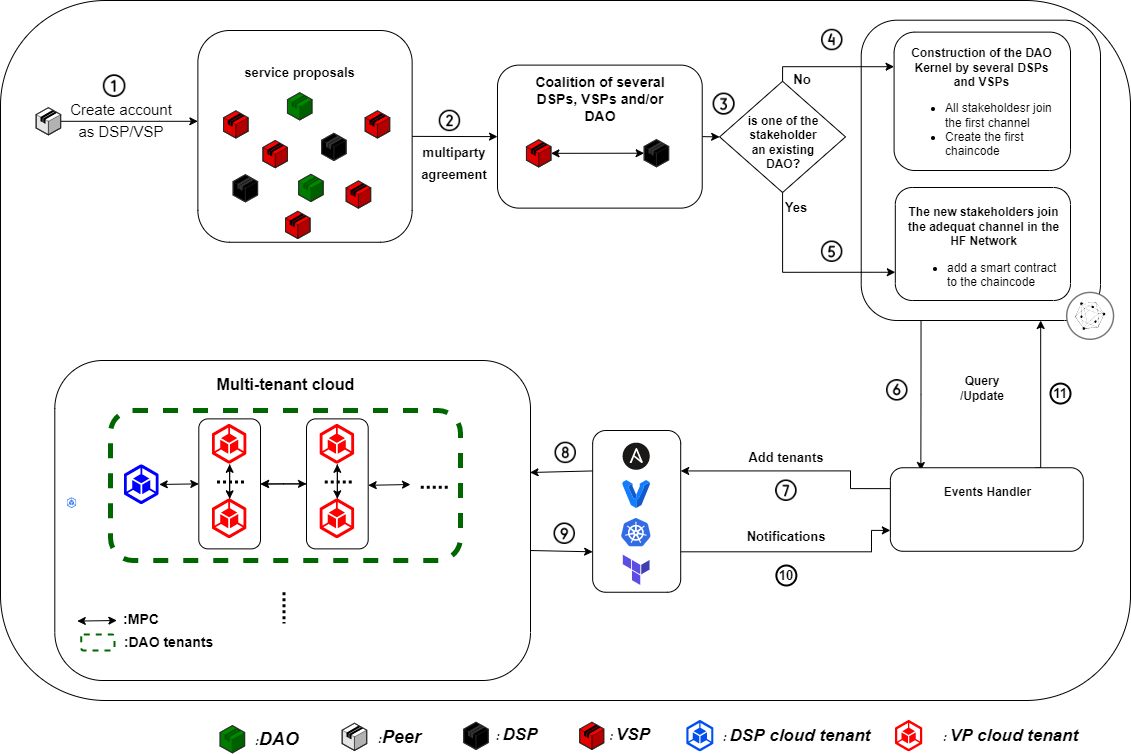
\includegraphics[width=\textwidth]{chart.png}
  \caption{Chart Flow }
\label{}
\end{figure*}



\begin{figure*}[!htb]
  \includegraphics[width=\textwidth,scale=.5]{cashflow.png}
  \caption{Cash Flow example with 4 parties.}
  \emph{Percentages are arbitrary set for the example. }
  \label{fig:cash}
\end{figure*}



\subsection{Data privacy}
As in \cite{damgaard2012multiparty}, a combination of Homomorphic encryption and multiparty computation will allow us to achieve a privacy-preserving framework to make our system even more data centric. It will enable our system to keep the data encrypted all the way through the computations and still have valuable results out of it.

\section{Some powerful aspects of the proposed architecture and  future work}\label{TrstRef}
As previously stated, our main goal is to make data driven projects preserve the right of privacy with no middle trusted authority. Data will never be decrypted during the whole process. Data owners will be able to make a profit from the final project as our vision is not to sell but to invest with data. One example of the possible business model will be a pay per use or subscription based, it all depends on the contract between the providers.\\
IoT infrastructures will rely significantly on our technology to offer a wide range of data to other parties for analysis and use while maintaining data privacy.\\
In terms of profit splitting, our system distributs profit group wise and according to each party's stake as defined in the chaincodes of each channel, see figure \ref{fig:cash} for a detailed tree graph describing the flow of profit.\\
As a future development, a user reputation system may be implemented. Parties can offer feedback on their interactions with a specific user by including a quality of experience mechanism, which will help us sanction poor conduct. This will boost user confidence, which is an important component of the online experience.



\section*{Conclusion}
Our system presents a functioning framework that allows anyone, and especially IoT infrastructure owners to invest their data in a distributed autonomous organisation amongst other service providers to further increase the value extracted from that data. This will benefit IoT device manufacturers since our future consists of more gadgets and sensors all over the cities and infrastructures, analytics services by having broader data point thus reducing the effects of 'small dataset curse' also known as overfitting, having real-time data to stay up to date. And the end users of course that will use the final service.
Our motivation is to have always our data protected but still making it work in the real world to improve services, applications and overall user experience.

\bibliographystyle{unsrt}
\bibliography{ref.bib}
\end{document}
